% Když budete cokoli psát: ukládejte starší verze vždy odděleně, abyste se 
% k nim mohli kdykoli vrátit. Kusy textu, které jste se rozhodli nepoužít, taky ukládejte do zvláštního souboru. Smazat se to dá vždycky, ale psát to znova je opruz. 

% A POŘÁD ZÁLOHUJTE. POŘÁD !!!

\documentclass[12pt, a4paper, oneside]{article} 
% velikost písma, stránky, typ dokumentu -- detaily viz literatura

\usepackage{czech} % nastavení češtiny
%\usepackage[latin2]{inputenc}
%\usepackage[cp1250]{inputenc} % pro win1250
\usepackage[utf8]{inputenc}
\usepackage{wrapfig} % nastavení obtékání textu
\usepackage{graphicx,amsmath} % nastavení grafiky, matematiky
\usepackage{subfig} % více obrázků vedle sebe 
\usepackage{float}
\usepackage{amsmath}
\usepackage{amssymb}
\usepackage{bbding}
\usepackage{enumitem}
\usepackage{multicol}
\usepackage{xfrac}
\usepackage{tocloft} %přidá tečky do obsahu ke kapitolám /sekcím 
\usepackage{pdflscape}
\renewcommand{\cftsecdotsep}{\cftdotsep}

\usepackage[bookmarksopen,colorlinks,plainpages=false,linkcolor=black,urlcolor=blue,citecolor=black,filecolor=black,menucolor=black,unicode=true]{hyperref}
%bookmarksopen -- open up bookmark tree 
%colorlinks -- zbarví odkazy (implicitně orámovaný nezbarvený text)
%urlcolor -- barva odkazů (implicitně magenta) 
%linkcolor=black -- barva odkazů v obsahu (implicitně red)


\usepackage{listings}
\usepackage{color}
\definecolor{lightgray}{rgb}{.9,.9,.9}
\definecolor{darkgray}{rgb}{.4,.4,.4}
\definecolor{purple}{rgb}{0.65, 0.12, 0.82}

\usepackage{parskip} %-- zapne americké odstavce v celé práci

\setlength{\textwidth}{170mm}


\setlength{\intextsep}{5mm} % nastavení mezery okolo obrázků

% nastavení příkazu >\figcaption pro popis čehokoli, jako by to byly obrázky 
\makeatletter   
\newcommand\figcaption{\def\@captype{figure}\caption}
\makeatother

% přejmenuje anglický název Reference na české Literatura


%\makeindex % příprava pro výrobu indexu (jestli ho chcete)

%%    VLNKA <fileinput>  KkSsVvZzOoUuAaIi        
% Defaultni  koncovka pro <fileinput> je  ".tex"
%FIXME: haze error
%\cstieon % Vypne chovani vlnky jako tvrde mezery v matematickem rezimu

%%%%%%%%%%%%%%%%%%%%%%%%%%%%%%%%%%%%%%%%%%%%%%%%%%%%%%%%%%%%%%%
%V PROSTŘEDÍ ROVNIC SE NESMÍ VYSKYTOVAT PRÁZDNÝ ŘÁDEK
%
%PROGRAMY VLNKA A CSINDEX SE MUSÍ SPUSTIT SAMOSTATNĚ
%%%%%%%%%%%%%%%%%%%%%%%%%%%%%%%%%%%%%%%%%%%%%%%%%%%%%%%%%%%%%%%

% definice příkazů 
\newcommand{\D}{\medskip \noindent} % nový odstavec v "americkém" formátování 
\newcommand{\B}{\textbf} %tučné písmo
\newcommand{\A}{\mathbf} %tučné písmo v matematickém režimu
\newcommand{\TO}{\ensuremath{\boldsymbol\Omega}} % tučný znak velké omega -- pro ohmy
\newcommand{\I}{\index}  % vytváří položku indexu (asi nepoužijete)
\newcommand{\Deg}[1][]{\ensuremath{{#1}^\circ}} % vysází značku stupně Celsia
\newcommand{\Def}{\footnotesize Definice: \normalsize}
\newcommand{\Pos}{\footnotesize Experiment: \normalsize}
\newcommand{\Odv}{\footnotesize Odvození: \normalsize}
\newcommand{\Vym}{\footnotesize Vymezení pojmu: \normalsize}
\newcommand{\Ob}{obrázek }
\newcommand{\It}{\textit}  % kurzíva
\newcommand{\M}{\mathrm}   % v prostředí rovnic nastaví normální písmo (místo kurzívy ) 
\newcommand{\F}{\footnotesize} % zmenšená velikost písma
\newcommand{\N}{\normalsize} % normální velikost písma
%\newcommand{\U}{\underline}  % podtržené písmo
\newcommand{\e}{\ensuremath} 
\newcommand{\Has}{\textcolor{green}{\CheckmarkBold}}
\newcommand{\NoHas}{\textcolor{red}{\XSolidBrush}}
% další příkaz se aplikuje, pouze, když jste v matematickém režimu

%\hyphenation{Pusť-me pla-tí hod-no-ty do-sa-dí-me za-da-né dal-ším}
% dělení slov, kdyby implicitní nevyhovovalo

\linespread{1.0} 
% řádkování 1,5x  
% použijete podle situace  

\unitlength=1mm % nastavení volby jednotek 


% konec hlavičky
%%%%%%%%%%%%%%%%%%%%%%%%%%%%%%%%%%%%%%%%%%%%%%%%%%%%%%%%%%%%%%%%%%%
%%%%%%%%%%%%%%%%%%%%%%%%%%%%%%%%%%%%%%%%%%%%%%%%%%%%%%%%%%%%%%%%%%%

\setlength{\hoffset}{-20mm}  % posun textu kvůli kroužkové vazbě  

\begin{document} % začátek textové části 

% titulní strana
\pagestyle{empty} % vynechá číslování
 
\voffset = -20mm % posun začátku textu výš
\enlargethispage{60mm} % zvětší oblast tisku pro tuto stránku   

\begin{center}
    \Large \B{LORRIS TOOLBOX \\ sada nástrojů pro vývoj a řízení robotů}
\end{center}
\vspace{5mm}
\setlength{\footskip}{0pt}
\setlength{\textheight}{750pt}

Lorris Toolbox je sada několika nástrojů, které mají společný cíl -- pomáhat při vývoji, ladění a řízení robotů a jiných elektronických zařízení.

{\large \B 1. Analyzér }
\begin{itemize}
    \item Soustřeďuje se na zobrazování dat z robota v grafické podobě
    \item Analyzér pro zobrazování používá tzv. widgety -- malá \uv{okna}, která zobrazují určitou část dat
    \item Widgety mají individuální nastavení a uživatel si je může umístit na libovolné místo na pracovní ploše
    \item Lorris obsahuje několik typů widgetů, například \It{ Číslo, Barva, Sloupcový bar, Kolo} (zobrazení úhlu v kružnici) či \It{Graf}.
    \item Pomocí widgetů lze sestavit rozhraní vyhovující prakticky jakémukoliv robotovi
    \item Analyzér je ideální pro snadné zobrazování dat z prvků, u kterých není vhodné jako výstup použít čísla -- například barevný senzor
    \item Některé widgety mohou posílat data i směrem do robota. Díky tomu je možné kromě zobrazování dat robota i ovládat
    \item Pozornost si zaslouží widget \uv{script}. Uživatel v něm může napsat vlastní script, který zpracovává příchozí data. Script může využít ostatní widgety a další části Lorris, díky tomu lze zobrazit takřka jakákoliv data.
\end{itemize}
\begin{center}
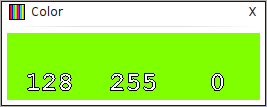
\includegraphics{img/color.png} \\
\It{Příklad: widget \uv{barva}}
\end{center}

\\{\large \B 2. Uživatelské prostředí pro programátor Shupito }

\begin{itemize}
    \item Shupito je programátor mikrokontrolérů. Na jeden konec programátoru se připojí čip, na druhý počítač -- bez programátoru nelze do mikrokontrolérů nahrát program.
    \item Lorris obsahuje uživatelské rozhraní pro ovládání Shupita -- zapisování programu, čtení a mazání paměti čipu a programování pojistek
\end{itemize}

\\{\large \B 3. Terminál }

\begin{itemize}
    \item Klasický terminál - zobrazuje příchozí data jako text nebo vypisuje byty jako hexadecimální čísla.
\end{itemize}

\\{\large \B 4. Proxy mezi sériovým portem a TCP socketem }

\begin{itemize}
    \item Vytvoří server připojený na sériový port - k tomuto portu je pak možné se připojit odkudkoliv z internetu
\end{itemize}

\newpage
\voffset = -30mm % posun začátku textu výš
\begin{center}
    \Large \B{PŘÍKLAD POUŽITÍ \\ Stavba robota, část 1: kostra}
\end{center}
\vspace{5mm}
Prvním krokem při stavbě robota je obvykle postavení kostry s motory. Tyto widgety slouží pro ovládání robota pomocí joysticku připojeného k PC, tak lze otestovat funkčnost a chování motorů.
\vspace{30mm}
\begin{center}
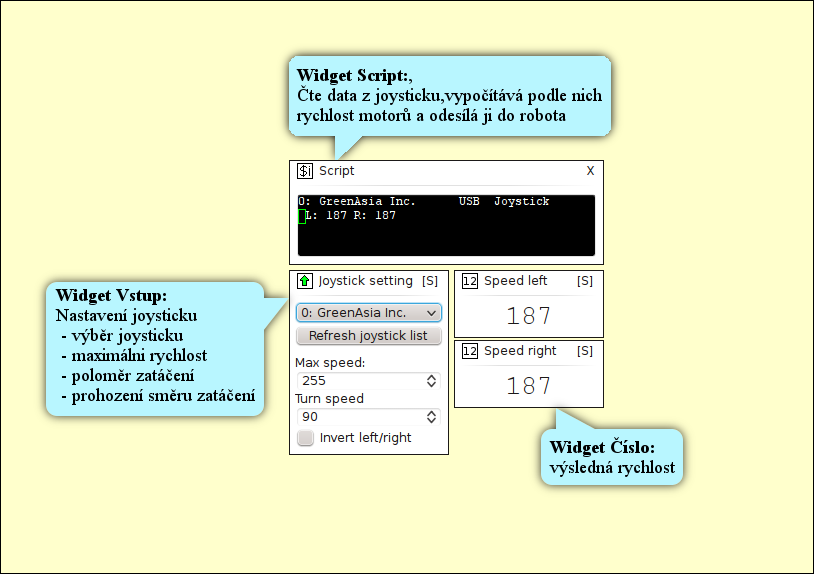
\includegraphics{img/joystick2.png}
\end{center}

\newpage
\voffset = -30mm % posun začátku textu výš
\begin{center}
    \Large \B{PŘÍKLAD POUŽITÍ \\ Stavba robota, část 2: senzory}
\end{center}
\vspace{5mm}
Dalším stupněm vývoje je přidání všech senzorů, podle kterých se robot může orientovat. Tato část je konceptována jako pohled shora na robota - widget \It{Script} tvoří tělo robota, na každém rohu je tlačítko signalizující náraz do mantinelu, u obou kol je enkodér, vepředu jsou dva ultrazvukové měřáky vzdálenosti a barevný senzor.
%\vspace{30mm}
\begin{center}
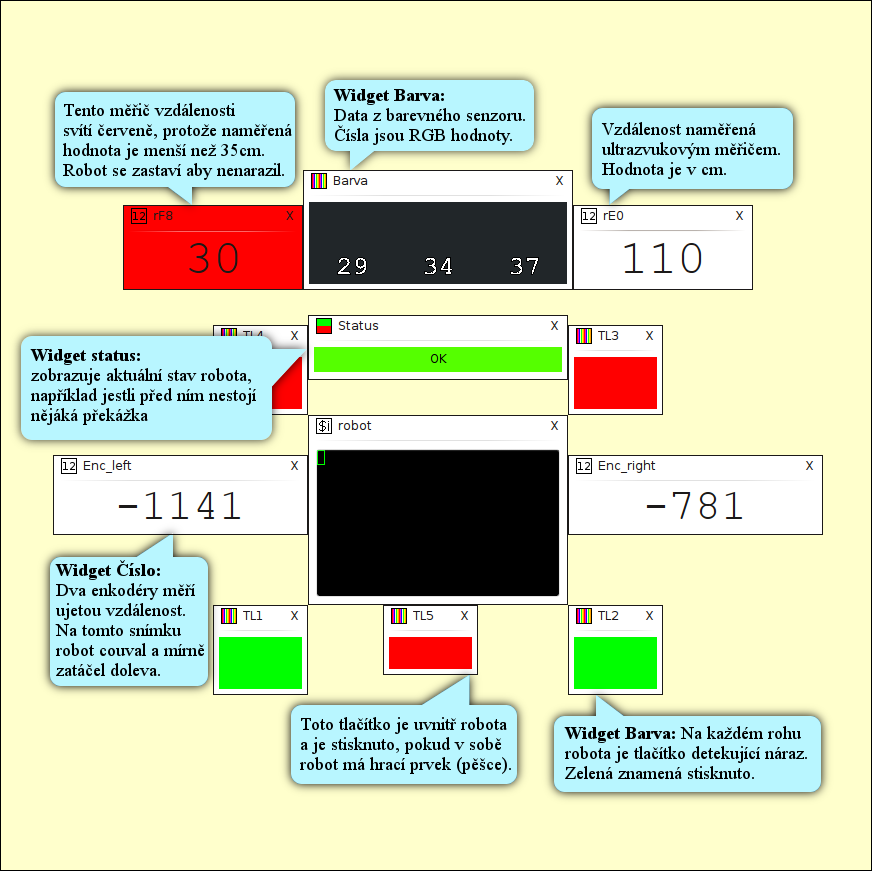
\includegraphics[scale=0.85]{img/sensors2.png}
\end{center}

\newpage
\begin{landscape}
\voffset = -30mm % posun začátku textu výš
\begin{center}
    \Large \B{PŘÍKLAD POUŽITÍ \\ Stavba robota, část 3: programování}
\end{center}
\vspace{5mm}
Poslední je vývoj samotného programu robota. V tomto příkladu používám jednoduché \uv{akce}, které robot postupně provádí. 

Každá akce má 3 hlavní parametry - směr jízdy, kdy se má robot zastavit a co má vykonat když se zastaví na cílovém místě. Všechny akce je možno rovnou měnit, bez nutnosti přeprogramovat robota.
%\vspace{30mm}
\begin{center}
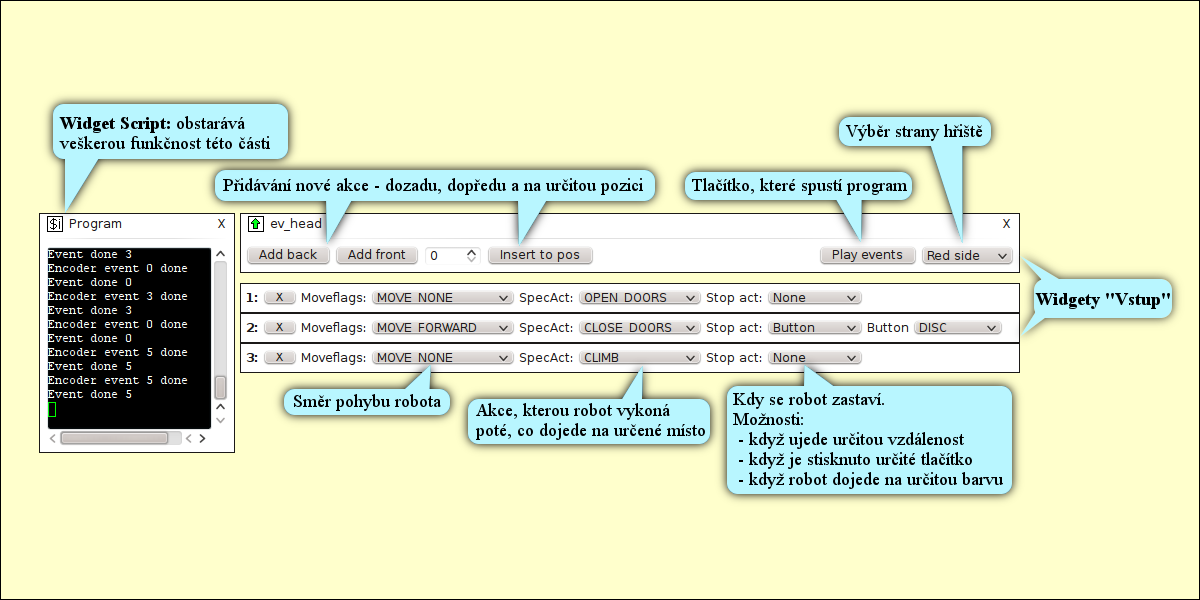
\includegraphics[scale=1]{img/control2.png}
\end{center}
\end{landscape}


\end{document}







